\documentclass[final, xcolor={table,dvipsnames},t]{beamer}

% ====================
% Packages
% ====================
\usepackage[T1]{fontenc}
\usepackage{lmodern}
\usepackage[orientation=portrait, size=custom, width=91.44, height=121.92, scale=0.94]{beamerposter}
\usetheme[Blue]{UVic}
\usepackage{graphicx}
\usepackage{caption}
\usepackage{booktabs}
\usepackage{tikz}
\usepackage{pgfplots}
\usepackage{amsmath,amssymb}
\pgfplotsset{compat=1.17}
\newcommand{\blu}{\color{UVicDarkBlue}}

%%%%%%%%%%%%%%%%%%%%%%%%%%%%%%%%%%%%%%%%%%%%%%%%%%%%%%%%%%%%%%%%%%%%%%%%%%%%%%
% Column environment setup
%%%%%%%%%%%%%%%%%%%%%%%%%%%%%%%%%%%%%%%%%%%%%%%%%%%%%%%%%%%%%%%%%%%%%%%%%%%%%%
\newlength{\sepwidthA}
\newlength{\colwidthA}
\setlength{\sepwidthA}{0.025\paperwidth}
\setlength{\colwidthA}{0.95\paperwidth}
\newcommand{\separatorcolumnA}{\begin{column}{\sepwidthA}\end{column}}

\newlength{\sepwidthB}
\newlength{\colwidthB}
\setlength{\sepwidthB}{0.020\paperwidth}
\setlength{\colwidthB}{0.305\paperwidth}
\newcommand{\separatorcolumnB}{\begin{column}{\sepwidthB}\end{column}}

%%%%%%%%%%%%%%%%%%%%%%%%%%%%%%%%%%%%%%%%%%%%%%%%%%%%%%%%%%%%%%%%%%%%%%%%%%%%%%
% Title
%%%%%%%%%%%%%%%%%%%%%%%%%%%%%%%%%%%%%%%%%%%%%%%%%%%%%%%%%%%%%%%%%%%%%%%%%%%%%%
\title{\VeryHuge Cost-Aware AgentRouter:\\ A Cheaper Coding-Agent Frontier}
\author{Ziming Dong$^{1}$, Ming Chen, Nhan Huynh, Jason Thomo$^{1}$}
\institute[shortinst]{$^{1}$Department of Computer Science, University of Victoria}

%%%%%%%%%%%%%%%%%%%%%%%%%%%%%%%%%%%%%%%%%%%%%%%%%%%%%%%%%%%%%%%%%%%%%%%%%%%%%%
% Footer
%%%%%%%%%%%%%%%%%%%%%%%%%%%%%%%%%%%%%%%%%%%%%%%%%%%%%%%%%%%%%%%%%%%%%%%%%%%%%%
\footercontent{
\href{mailto:dzm1098@uvic.ca}{dzm1098@uvic.ca}
  \hfill
  CSC 504 \quad Group 13 \textemdash{} Project repo on UVic GitLab
  \hfill
  University of Victoria }

\begin{document}
%%%%%%%%%%%%%%%%%%%%%%%%%%%%%%%%%%%%%%%%%%%%%%%%%%%%%%%%%%%%%%%%%%%%%%%%%%%%%%
% UVic CS logo in top-left corner
%%%%%%%%%%%%%%%%%%%%%%%%%%%%%%%%%%%%%%%%%%%%%%%%%%%%%%%%%%%%%%%%%%%%%%%%%%%%%%
\addtobeamertemplate{headline}{}{}

\begin{frame}[t]

%%%%%%%%%%%%%%%%%%%%%%%%%%%%%%%%%%%%%%%%%%%
% Small CS logo placed top-left of body, before motivation banner
%%%%%%%%%%%%%%%%%%%%%%%%%%%%%%%%%%%%%%%%%%%
\begin{tikzpicture}[remember picture,overlay]
    \node [anchor=north west, inner sep=0cm]
      at ([xshift=1.0cm,yshift=-1.8cm]current page.north west)
      {
\includegraphics[height=3.2cm]{logos/uvic_cs_logo.jpg}};
\end{tikzpicture}

%%%%%%%%%%%%%%%%%%%%%%%%%%%%%%%%%%%%%%%%%%%
% Group number + members, top-right (required by spec)
%%%%%%%%%%%%%%%%%%%%%%%%%%%%%%%%%%%%%%%%%%%
\begin{tikzpicture}[remember picture,overlay]
    \node [anchor=north east, inner sep=0cm, align=right, text=white]
      at ([xshift=-1.5cm,yshift=-1.6cm]current page.north east)
      {{\Large\textbf{Group 13}}\\[0.4ex]
       {\normalsize Ziming Dong \;\textbar\; Nhan Huynh \;\textbar\; Ming Chen \;\textbar\; Jason Thomo}};
\end{tikzpicture}

%%%%%%%%%%%%%%%%%%%%%%%%%%%%%%%%%%%%%%%%%%%
% TOP BANNER
%%%%%%%%%%%%%%%%%%%%%%%%%%%%%%%%%%%%%%%%%%%
\begin{columns}[t]
    \separatorcolumnA
    \begin{column}{\colwidthA}

        \begin{alertblock}{Motivation \textemdash{} Should teams route between AI coding agents to cut cost?}
        \Large
        Teams increasingly run several AI coding agents (Codex, Copilot, Cursor, Devin, Claude) side by side. Their subscription and usage prices differ \textbf{several-fold} \textemdash{} yet teams usually pick one agent out of habit, not per task.

        \vspace{0.5ex}
        \textbf{Our question:} Can we learn an offline router on observational GitHub data (AIDev, \(\sim\)932k PRs) that picks the right agent per task, and \emph{value} that policy without ever running a live A/B test?
    
        \end{alertblock}
    \end{column}
    \separatorcolumnA
\end{columns}

%%%%%%%%%%%%%%%%%%%%%%%%%%%%%%%%%%%%%%%%%%%
% THREE-COLUMN MAIN BODY
%%%%%%%%%%%%%%%%%%%%%%%%%%%%%%%%%%%%%%%%%%%
\begin{columns}[t]
\separatorcolumnB
%%%%%%%%%%%%%%%%%%%%%%%%%%%%%%%%%%%%%%%%%%%
% LEFT COLUMN
%%%%%%%%%%%%%%%%%%%%%%%%%%%%%%%%%%%%%%%%%%%
\begin{column}[T]{\colwidthB}

    \begin{block}{Research Questions}
    \begin{itemize}\itemsep
        \item \textbf{RQ1.} Do the five agents show different merge rates across task categories?
        \item \textbf{RQ2.} How well can a regressor predict per-agent success from task/repo features, and does model capacity help?
        \item \textbf{RQ3.} Can a cost-aware router improve the cost-quality trade-off over always-best-agent, and which signal achieves it?
    \end{itemize}
    \end{block}
    

    \begin{block}{Dataset \& Setup}
    \textbf{AIDev} [Li et al.\ 2026]: 932k agentic PRs, 5 commercial agents, public GitHub.

    \textbf{Balanced corpus:} down-sampled to \textbf{25,580 PRs} (5,116/agent) so minority agents are learnable.

    \textbf{Splits:} 70/15/15 grouped by \texttt{repo\_id} (no repo crosses splits).

    \textbf{Target:} graded \texttt{success} label (merged $=1$, open $=0.3$, closed $=0$); MAE metric.
    \end{block}


    \begin{block}{Reduced-Leakage Features}
    Title and body are written by the agent \emph{after} it acts \textemdash{} \textbf{post-treatment}. v2 drops the body and all body-derived features; it keeps:
    \begin{itemize}
        \item Cleaned title (agent tokens stripped)
        \item Repo metadata: language, \(\log\) stars/forks
        \item \texttt{has\_issue}, \texttt{task\_type}, agent one-hot
    \end{itemize}
    \end{block}


    \begin{block}{Normalized Per-PR Cost}
    \centering
    \begin{tabular}{l@{\hspace{2.5cm}}r}
    \toprule
    Agent & \$ / PR \\
    \midrule
    Copilot         & 1.10 \\
    OpenAI\_Codex   & 3.85 \\
    Cursor          & 3.85 \\
    Devin           & 4.50 \\
    Claude\_Code    & 4.80 \\
    \bottomrule
    \end{tabular}
    \\[0.6ex]
    \small\raggedright Method comparison is \emph{price-invariant}: a new scenario only rescales the cost axis.
    \end{block}

    \begin{block}{How AI Helped / Didn't}
    \textbf{Helped:} code and Latex scaffolding, figure layout, related-work search, prose drafting and around 90\% code writing.

    \textbf{Didn't:} every number comes from our own runnable pipeline, not AI text; and AI first kept the leaky PR body until we audited what the model keyed on.
    \end{block}

\end{column}
\separatorcolumnB
%%%%%%%%%%%%%%%%%%%%%%%%%%%%%%%%%%%%%%%%%%%
% MIDDLE COLUMN
%%%%%%%%%%%%%%%%%%%%%%%%%%%%%%%%%%%%%%%%%%%
\begin{column}[T]{\colwidthB}

    \begin{block}{Agents vs.\ Task Category}
    Codex's merge rate ranges \textbf{84-89\%} against \textbf{48-66\% for Copilot} across the eight most common task types: agents are not interchangeable.
    \begin{figure}
        \centering
        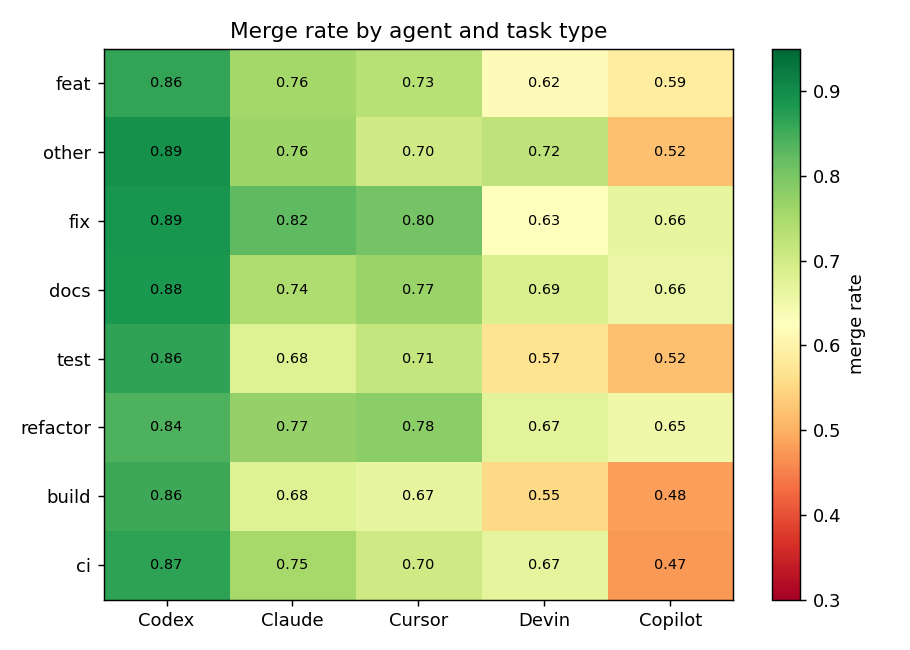
\includegraphics[width=0.80\textwidth]{figures/fig2_agent_tasktype_heatmap.png}
    \end{figure}
    But Codex leads in \emph{every} common cell: heterogeneity is real in level yet \textbf{weak as a routing signal}.
    \end{block}
    

    \begin{block}{Per-Agent Success}
    \centering
    \begin{tabular*}{0.9\linewidth}{@{\extracolsep{\fill}}lr}
    \toprule
    Model (v2 title+repo features) & test MAE \\
    \midrule
    per-agent-mean baseline & 0.331 \\
    Ridge (linear)          & 0.306 \\
    XGBoost (tuned)         & \textbf{0.306} \\
    \bottomrule
    \end{tabular*}
    \raggedright
    \textbf{Linear matches XGBoost} \textemdash{} \emph{signal-limited}. Only \textbf{agent} and \textbf{language} carry out-of-sample signal.
    \end{block}


    \begin{block}{Selection Bias}
    Propensity model predicts \emph{acting agent} at \textbf{0.36 vs 0.20 chance}.
    \begin{figure}
    \centering
    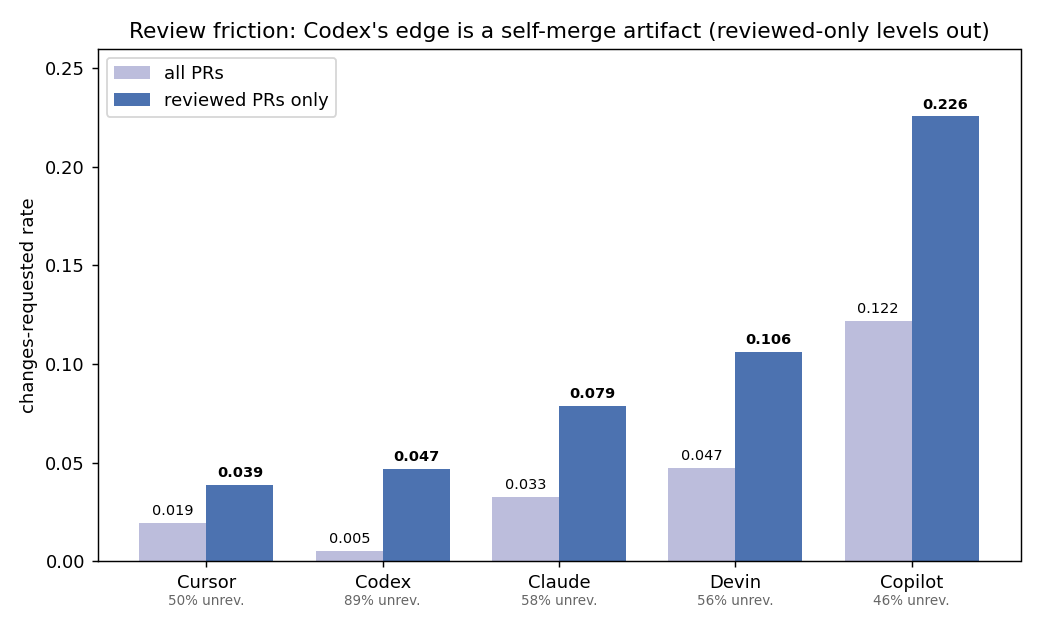
\includegraphics[width=0.64\textwidth]{figures/fig5_quality.png}
    \end{figure}
    \textbf{89\% of Codex PRs are self-merged.} Reviewed-only: Codex collapses (0.005\,\(\to\)\,0.047); Cursor (0.039) cleaner.
    \end{block}

    \begin{block}{What's Next}
    \begin{itemize}
        \item Time-based split for temporal drift; survival label for still-open PRs.
        \item RouteLLM and peers as runnable baselines on AIDev (time-limited here).
        \item Quality labels beyond merge: reviews, reverts, tests.
    \end{itemize}
    \end{block}

\end{column}
\separatorcolumnB
%%%%%%%%%%%%%%%%%%%%%%%%%%%%%%%%%%%%%%%%%%%
% RIGHT COLUMN
%%%%%%%%%%%%%%%%%%%%%%%%%%%%%%%%%%%%%%%%%%%
\begin{column}[T]{\colwidthB}

    \begin{block}{A Cheaper Pareto Frontier}
    \begin{figure}
    \centering
    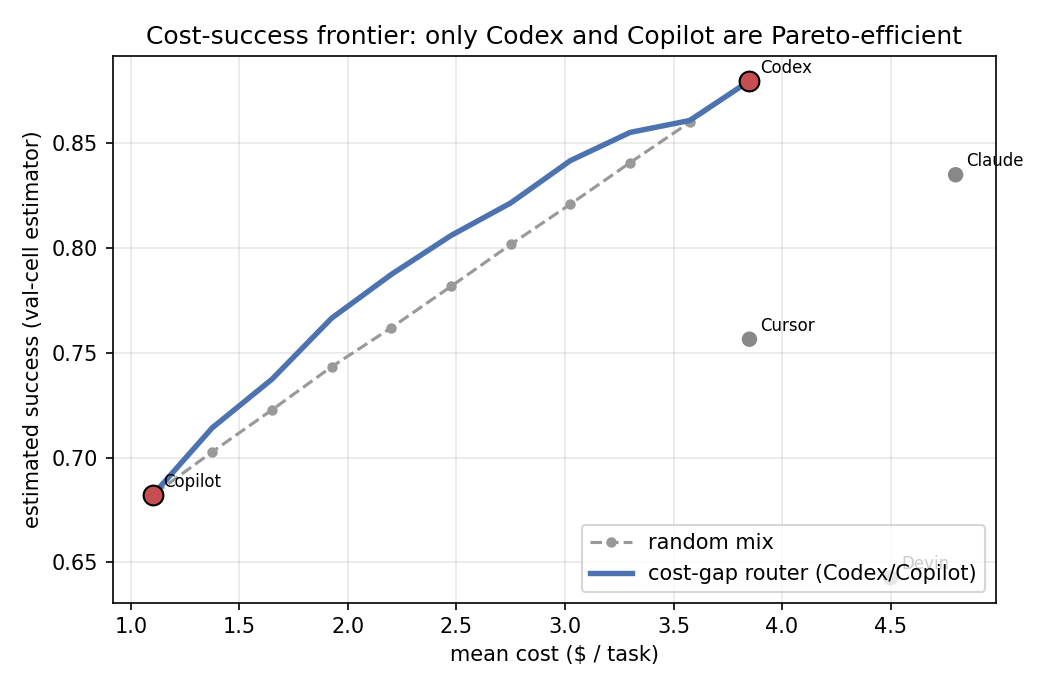
\includegraphics[width=0.78\textwidth]{figures/fig9_cost_router_pareto.png}
    \end{figure}
    Under our cost scenario and the merge metric, \textbf{only Codex and Copilot} are Pareto-efficient; the cost-gap router trades along the Codex$\to$Copilot edge. \textbf{Success at matched cost}:
    \centering
    \begin{tabular*}{0.95\linewidth}{@{\extracolsep{\fill}}lrrr}
    \toprule
    Mean cost & random & instance & \textbf{cost-gap} \\
    \midrule
    \$3.85 (always-Codex) & 0.880 & 0.880 & 0.880 \\
    \$3.30 ($-14\%$)      & 0.841 & 0.839 & \textbf{0.855} \\
    \$2.75 ($-29\%$)      & 0.801 & 0.803 & \textbf{0.821} \\
    \$2.20 ($-43\%$)      & 0.761 & 0.763 & \textbf{0.787} \\
    \bottomrule
    \end{tabular*}
    \raggedright
    \textbf{Bottom line:} keep \textbf{93\% of always-Codex's success at 29\% lower cost}. The edge is \emph{significant} under direct-method and two-level bootstraps, \emph{positive but not significant} under high-variance IPW/DR.
    \end{block}


    \begin{alertblock}{Key Takeaways}
    \begin{itemize}
        \item \textbf{Routing wins on cost, not success}: \(\sim\)93\% of merge rate at 29\% lower cost.
        \item \textbf{Success ranking not identifiable}: the \(\sim\)4-pt estimator spread exceeds the 1--2-pt policy gaps.
        \item \textbf{``Best'' \(\approx\) ``most-used''}: always-best and most-popular pick the same agent \textbf{99\%} of the time.
    \end{itemize}
    \end{alertblock}

    \begin{block}{What We Learned}
    \begin{itemize}
        \item \textbf{Leakage hides in provenance.} The PR body carries agent signatures (footers, co-authored-by); mined ``input'' text is often written \emph{after} the outcome.
        \item \textbf{In-sample importance lies.} Split gain put 84\% on the title, yet permutation and ablation show it carries almost no out-of-sample value.
        \item \textbf{The mining trap.} A raw merge leaderboard reads a self-merge usage pattern as capability; adjust for assignment before trusting an observational label.
    \end{itemize}
    \end{block}

    \begin{block}{}
    \scriptsize
    \setlength{\parindent}{0pt}
    [1] H. Li, H. Zhang, A. E. Hassan. \emph{AIDev: Studying AI Coding Agents on GitHub}. arXiv:2602.09185, 2026.\\[0pt]
    [2] I. Ong et al. \emph{RouteLLM}. ICLR, 2025.\\[0pt]
    [3] E. Kalliamvakou et al. \emph{Promises and Perils of Mining GitHub}. EMSE, 2016.
    \end{block}

\end{column}
\separatorcolumnB
\end{columns}
\end{frame}
\end{document}